\documentclass[10pt,a4paper]{article}
\usepackage[utf8]{inputenc}
\usepackage[T1]{fontenc}
\usepackage{geometry}
 \geometry{
    a4paper,
    total={210mm,297mm},
    left=5mm,
    right=5mm,
    top=15mm,
    bottom=15mm
 }
\usepackage{amsmath}
\usepackage{dependencies/caratula,dependencies/aed2-symb,dependencies/aed2-itef,dependencies/aed2-tad, dependencies/aed2-helper}
\usepackage[spanish]{babel}
\usepackage{fancyhdr}
\usepackage{algorithm2e}
\usepackage{algpseudocode}
\usepackage{listings}
\usepackage{color}     % para snipets de codigo coloreados
\usepackage{xcolor}
\usepackage{fancybox}  % para el sbox de los snipets de codigo
\usepackage[pdftex]{graphicx}

\usepackage{caption}
\usepackage{subcaption}
\usepackage{float}
\usepackage{lastpage}
\usepackage{afterpage}


% definiciones

\newtheorem{theorem}{Teorema}[section]
\newtheorem{lemma}[theorem]{Lema}
\newtheorem{proposition}[theorem]{Proposici\'on}
\newtheorem{corollary}[theorem]{Corolario}

\newcommand{\Var}{\textbf{var }}
\newcommand{\True}{\textbf{true }}
\newcommand{\False}{\textbf{false }}
\newcommand{\Break}{\textbf{break }}

\newenvironment{proof}[1][Demostraci\'on]{\begin{trivlist}
\item[\hskip \labelsep {\bfseries #1}]}{\end{trivlist}}
\newenvironment{definition}[1][Definici\'on]{\begin{trivlist}
\item[\hskip \labelsep {\bfseries #1}]}{\end{trivlist}}
\newenvironment{example}[1][Ejemplo]{\begin{trivlist}
\item[\hskip \labelsep {\bfseries #1}]}{\end{trivlist}}
\newenvironment{remark}[1][Observaci\'on]{\begin{trivlist}
\item[\hskip \labelsep {\bfseries #1}]}{\end{trivlist}}

\definecolor{litegrey}{gray}{0.94}

\newenvironment{codesnippet}{%
	\begin{Sbox}\begin{minipage}{\textwidth}\sffamily\small}%
	{\end{minipage}\end{Sbox}%
		\begin{center}%
		\vspace{-0.4cm}\colorbox{litegrey}{\TheSbox}\end{center}\vspace{0.3cm}}

\lstset{frame=tb,
	  language=Java,
	  aboveskip=3mm,
	  belowskip=3mm,
	  showstringspaces=false,
	  columns=flexible,
	  basicstyle={\scriptsize\ttfamily},
	  numberstyle=\tiny\color{gray},
	  keywordstyle=\color{blue},
	  commentstyle=\color{green},
	  stringstyle=\color{red},
	  breaklines=true,
	  breakatwhitespace=true,
	  tabsize=3,
	  numbers=left,
	  numbersep=15pt,
	  numberfirstline = false
	}


\begin{document}

% **************************************************************************
%
%  Package 'caratula', version 0.2 (para componer caratulas de TPs del DC).
%
%  En caso de dudas, problemas o sugerencias sobre este package escribir a
%  Nico Rosner (nrosner arroba dc.uba.ar).
%
% **************************************************************************



% ----- Informacion sobre el package para el sistema -----------------------

\NeedsTeXFormat{LaTeX2e}
\ProvidesPackage{caratula}[2003/4/13 v0.1 Para componer caratulas de TPs del DC]


% ----- Imprimir un mensajito al procesar un .tex que use este package -----

\typeout{Cargando package 'caratula' v0.2 (21/4/2003)}


% ----- Algunas variables --------------------------------------------------

\let\Materia\relax
\let\Submateria\relax
\let\Titulo\relax
\let\Subtitulo\relax
\let\Grupo\relax


% ----- Comandos para que el usuario defina las variables ------------------

\def\materia#1{\def\Materia{#1}}
\def\submateria#1{\def\Submateria{#1}}
\def\titulo#1{\def\Titulo{#1}}
\def\subtitulo#1{\def\Subtitulo{#1}}
\def\grupo#1{\def\Grupo{#1}}
\def\abstract#1{\def\Abstract{#1}}
\def\keywords#1{\def\Keywords{#1}}

% ----- Token list para los integrantes ------------------------------------

\newtoks\intlist\intlist={}


% ----- Comando para que el usuario agregue integrantes

\def\integrante#1#2#3{\intlist=\expandafter{\the\intlist
    \rule{0pt}{1.2em}#1&#2&\tt #3\\[0.2em]}}


% ----- Macro para generar la tabla de integrantes -------------------------

\def\tablaints{%
    \begin{tabular}{|l@{\hspace{4ex}}c@{\hspace{4ex}}l|}
        \hline
        \rule{0pt}{1.2em}Integrante & LU & Correo electr\'onico\\[0.2em]
        \hline
        \the\intlist
        \hline
    \end{tabular}}

% ----- Macro para generar la parte reservada para la c?tedra -------------------------

\def\tablacatedra{%
    \\
    \textbf{Reservado para la c\'atedra}\par\bigskip
    \begin{tabular}{|c|c|c|}
        \hline
        \rule{0pt}{1.2em}Instancia & Docente & Nota\\[0.2em]
        \hline
        \rule{0pt}{1.2em}Primera entrega & \phantom{mmmmmmmmmmmmmmmmmm} & \phantom{mmmmmm} \\
        \hline
        \rule{0pt}{1.2em}Segunda entrega & & \\
        \hline
    \end{tabular}}

% ----- Codigo para manejo de errores --------------------------------------

\def\se{\let\ifsetuperror\iftrue}
\def\ifsetuperror{%
    \let\ifsetuperror\iffalse
    \ifx\Materia\relax\se\errhelp={Te olvidaste de proveer una \materia{}.}\fi
    \ifx\Titulo\relax\se\errhelp={Te olvidaste de proveer un \titulo{}.}\fi
    \edef\mlist{\the\intlist}\ifx\mlist\empty\se%
    \errhelp={Tenes que proveer al menos un \integrante{nombre}{lu}{email}.}\fi
    \expandafter\ifsetuperror}


% ----- Reemplazamos el comando \maketitle de LaTeX con el nuestro ---------

\def\maketitle{%
    \ifsetuperror\errmessage{Faltan datos de la caratula! Ingresar 'h' para mas informacion.}\fi
    \thispagestyle{empty}
    \begin{center}
    \vspace*{\stretch{2}}
    {\LARGE\textbf{\Materia}}\\[1em]
    \ifx\Submateria\relax\else{\Large \Submateria}\\[0.5em]\fi
    \par\vspace{\stretch{1}}
    {\large Departamento de Computaci\'on}\\[0.5em]
    {\large Facultad de Ciencias Exactas y Naturales}\\[0.5em]
    {\large Universidad de Buenos Aires}
    \par\vspace{\stretch{3}}
    {\Large \textbf{\Titulo}}\\[0.8em]
    {\Large \Subtitulo}
    \par\vspace{\stretch{3}}
    \ifx\Grupo\relax\else\textbf{\Grupo}\par\bigskip\fi
    \tablaints
    \vspace*{\stretch{3}}
    \medskip
    \tablacatedra
    \end{center}
    
    \vspace*{\stretch{2}}
	\textbf{Comentarios del corrector: }
    \newpage
    }

\newpage

\tableofcontents
\newpage

\section{Introducción}





\newpage

\section{Desarrollo}

La implementación del traceroute con el cual se realizó este trabajo se basa en la técnica de TTls incrementales. Comenzando con TTL = 1 (el router más cercano, primer salto) mandar paquetes Echo Requeste al destino mientras se sigan recibiendo mensajes de Time Exceeded. Por cada uno se recibe se incrementa en 1 el TTL hasta recibir un Echo Reply o en su defecto hasta el máximo TTL especificado en el protocolo IP. \\
Para asegurarnos de obtener una muestra amplia, se envían por cada TTL rafagas de 30 paquetes. Cada uno en caso de ser respondido, devuelve una IP y el RTT hasta eso salto. Se determina cuál es la dirección que más veces responde en ese salto y se obtiene un promedio de los RTT que reportó. Este valor es el que guardamos para cada ese salto.\\

Tras la recepción de un Echo Reply, se calcula 
$\Delta RTT_{i}=RTT_{i}-RTT_{i-1}$ que determina el RTT de 
la conexión entre cada salto. En el caso en el que se 
observe la anomalía en la cual se tarda menos en enviar un 
paquete a un salto más lejano, se descarta este 
$deltaRTT$. Como una red puede definirse recursivamente a 
partir de dos enlaces, podemos quitar el $i-esimo$ 
router/salto con $deltaRTT = RTT_{i}-max{RTT_{j}}, j < i$, 
aplanando así la red. De esta manera se es consistente con 
las leyes de la física.\\

Una vez determinado los RTT entre saltos, se calcula su promedio $\overline{RTT}$ y desvío standard $\sigma$. Esto se utilizan para el análisis estadístico de los outliers.\\

Como las conexiones intercontinentales deberían ilustrar saltos empinados en relación a los locales,se espera que estos seean represnetados como puntos/datos fuera de cierto patron observado en la muestra.
Para ello, nos basamos en el descarte de outliers propuesto por Cibala \cite{Cimbala}. 
Primero calculamos el desvío absoluto $\delta_{i}=|\delta_{i}-\overline{RTT}|$ para cada salto   $\Delta_{i}$.
Luego calculamos $ZRTT_{i}=\delta_{i}/\sigma$. Tomamos el que máximice $ZRTT$ entre todos los saltos y lo comparamos con la función Tao de Thompson evaluada en $n = |saltos|$ (saltos válidos como se propuso arriba), utilizando la tabla provista en la publicación.\\

\begin{itemize}
\item Si $ZRTT_{i} > \tau$, se etiqueta al salto de ttl $i$ como un outlier, y en consecuencia posible salto intercontinental y se itera sobre el resto de los saltos.
\item Caso contrario no hay más outliers ya que compara al máxima diferencia.
\end{itemize}

Comprobaremos experimentalmente el grado de acierto de este método de descarte de outliers colocándolo en contexto con los saltos subacuáticos buscados en el presente trabajo.\\


\subsection{Implementación}

Se implementó lo detallado en la subsección anterior gracias a la librería Scapy de Python \cite{Scapy}. Haciendo uso de la función sr (send and recieve) se envían paquetes \textit{Echo Request} y espera la respuesta. Para acotar el tiempo de esta, se introduce un timeout cuyo valor por defecto de un segundo. Se envían 30 paquetes por cada TTL, se calcula el de mayor aparición en cada caso y su promedio.\\

Almacenando esta información en un arreglo/diccionario se calcula los $\Delta RTT$, promedio y desvío standard con la libreria \textit{numpy} y luego se determinan los outliers como se especifica arriba.\\

La herramienta imprime en pantalla para cada TTL o salto, el $\overline{RTT_{i}}$, $\delta_{i}$ y si es outlier. 

\subsection{Condiciones de experimentación e hipótesis}

Se experimentaron enviando paquets a 4 universidades de 3 continentes (Norte América, Europa y Asia). La razon por la cual se testea el enlace a universidades es porque es muy probable que estas contesten los pedidos.\\

Se esperan al menos dos saltos intercontinentales en todos los casos, con notorias diferencias respecto a otros saltos. Tambien se espera que el RTT hasta Asia sea mayor que a Norte América y que a mayor cantidad de routers que respondan mayor será la precisión en tiempo y ubicación de la ruta trazada por el intercambio de mensajes ICMP.



\newpage

\section{Experimentación y Resultados}

\subsection{Africa}


\newpage
\subsection{Norte América}

En esta instancia de experimentaci'on vamos a analizar las rutas a la universidad de UNAM, ubicada en Mexico, utilizando la direcci'on \textit{unam.edu}. 

\begin{tabular}{ |p{1cm}||p{3cm}|p{2cm}|p{2cm}|p{1.5cm}|  }
 \hline
 \multicolumn{5}{|c|}{Traceroute a UNAM} \\
 \hline
 \textit{TTL} & \textit{IP}  & \textit{RTT} & $\delta$\textit{RTT} & Outlier? \\
 \hline
1    &    192.168.1.1    &     2.43 ms      &     -           &     \\               
2    &    Sin respuesta              &    -             &    -           &          \\                  
3     &   Sin respuesta              &    -            &     -         &        \\               
4    &    Sin respuesta               &    -            &     -          &        \\                   
5    &    Sin respuesta                &   -            &     -          &        \\                
6     &   200.89.161.85   &    19.59 ms     &     17.17 ms   &        \\              
7     &   200.89.165.197  &    20.53 ms     &     0.94 ms   &        \\            
8    &    200.89.165.222  &    22.96 ms     &     2.43 ms   &      \\               
9    &    Sin respuesta               &    -            &     -         &         \\                 
10   &    64.215.103.74    &   155.34 ms     &    132.38 ms  &  Outlier  \\    
11   &    159.63.49.142    &   192.17 ms    &     36.84 ms    &           \\              
12   &    201.140.112.97   &   184.71 ms    &     -         &           \\                
13   &    201.148.69.177   &   193.2 ms     &     1.03 ms         &      \\                    
14   &    132.247.237.217  &   184.7 ms      &    -         &           \\                 
15   &    132.247.237.189  &   183.25 ms    &     -         &          \\                  
16    &   132.247.70.37    &   176.05 ms     &    -        &       \\   
 \hline
\end{tabular}

\smallskip
    
\begin{figure}[H]
\centering
\caption{UNAM delta RTTs y ZRTT}
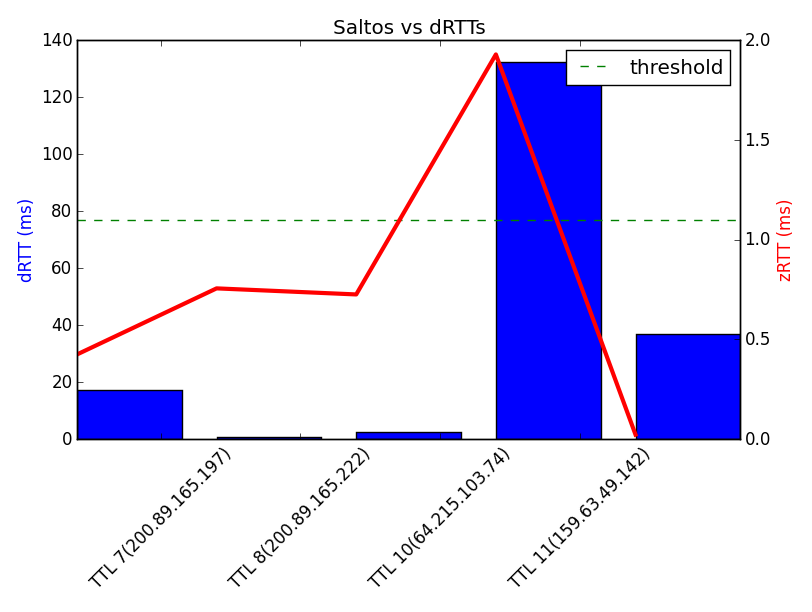
\includegraphics[width=0.55\textwidth]{modules/unam_rtts_2}
 \label{fig:unam_rtts_2}
\end{figure}

\begin{figure}[H]
\centering
\caption{UNAM RTTs por salto}
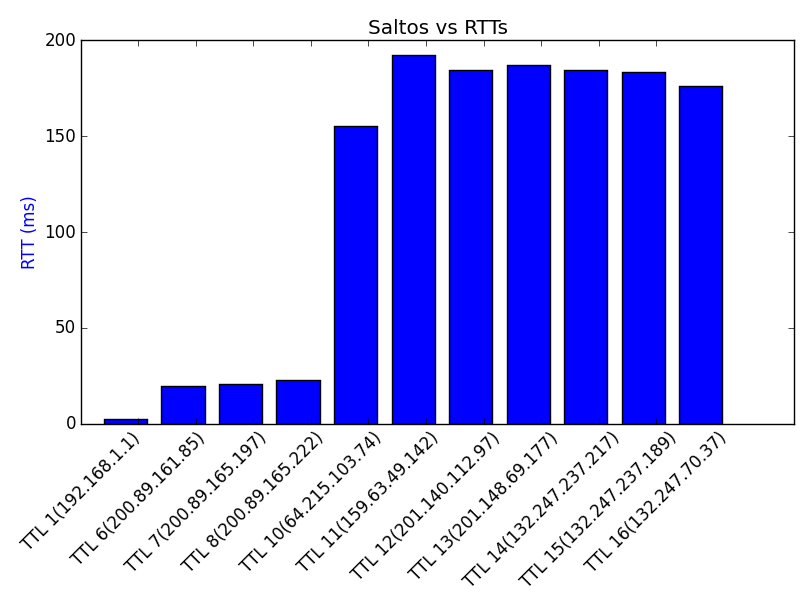
\includegraphics[width=0.55\textwidth]{modules/unam_rtts_1}
 \label{fig:unam_rtts}
\end{figure}

Mencionar que pasa por USA
\begin{figure}[H]
\centering
\caption{Ruta a UNAM}
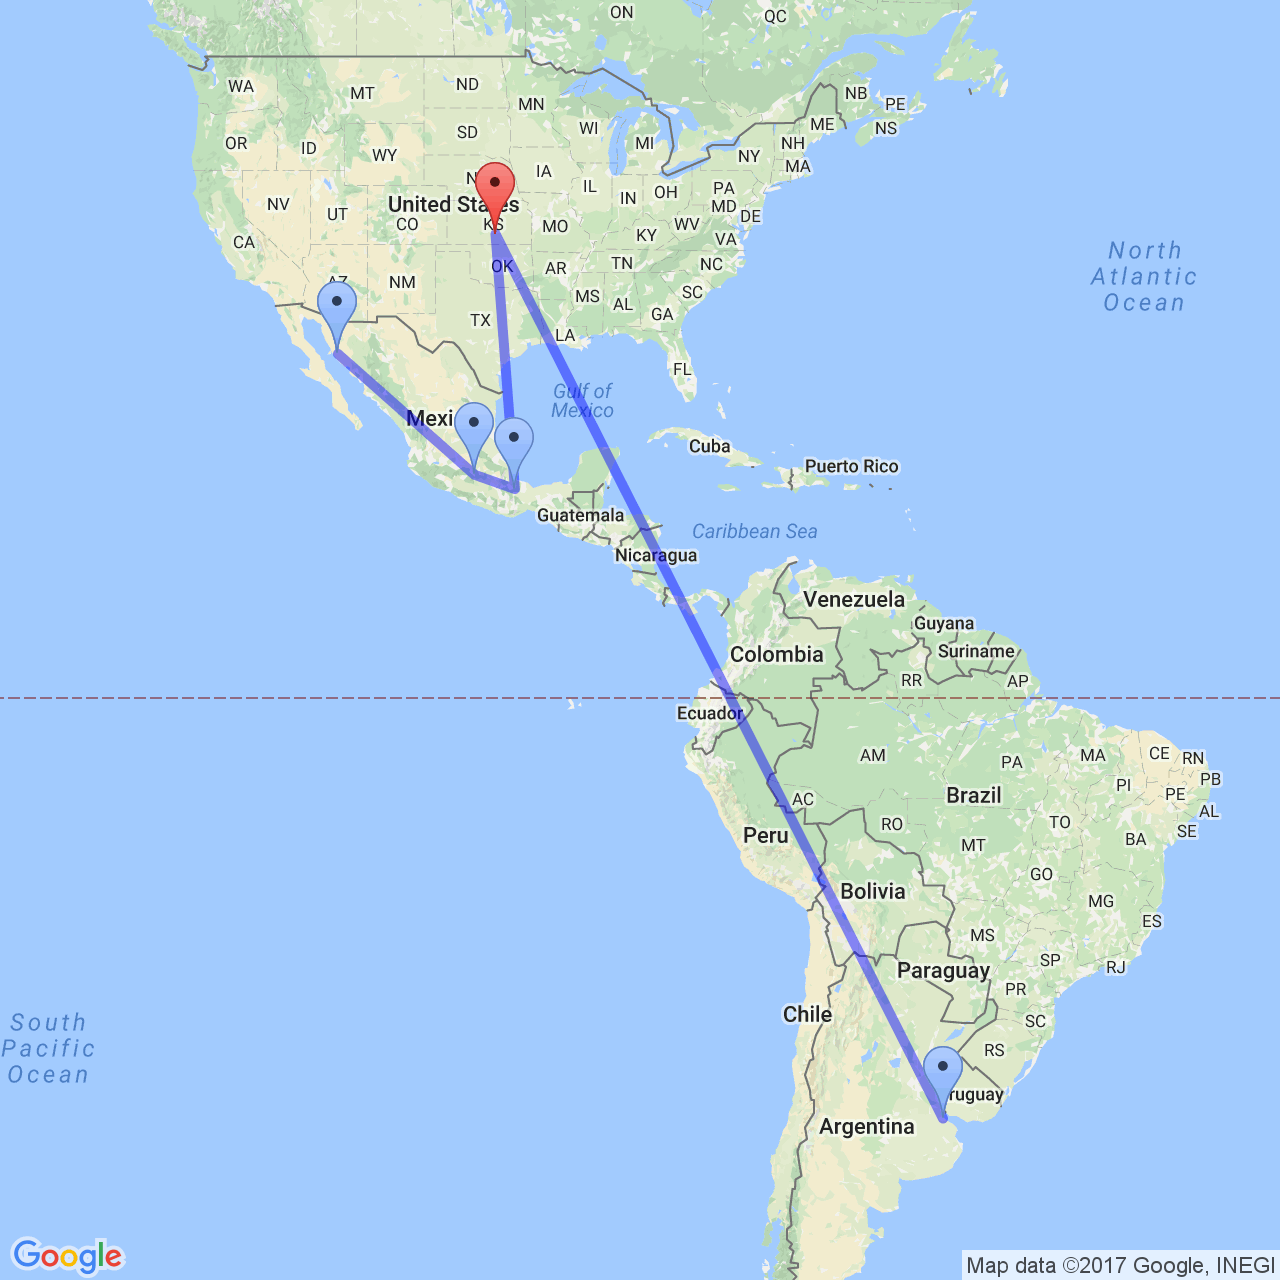
\includegraphics[width=0.55\textwidth]{modules/unam_path_1}
 \label{fig:ruta_unam_1}
\end{figure}

LPM UNAM no queda en el desierto de sonora, geolocation fallo
\begin{figure}[H]
\centering
\caption{Ruta en Mexico}
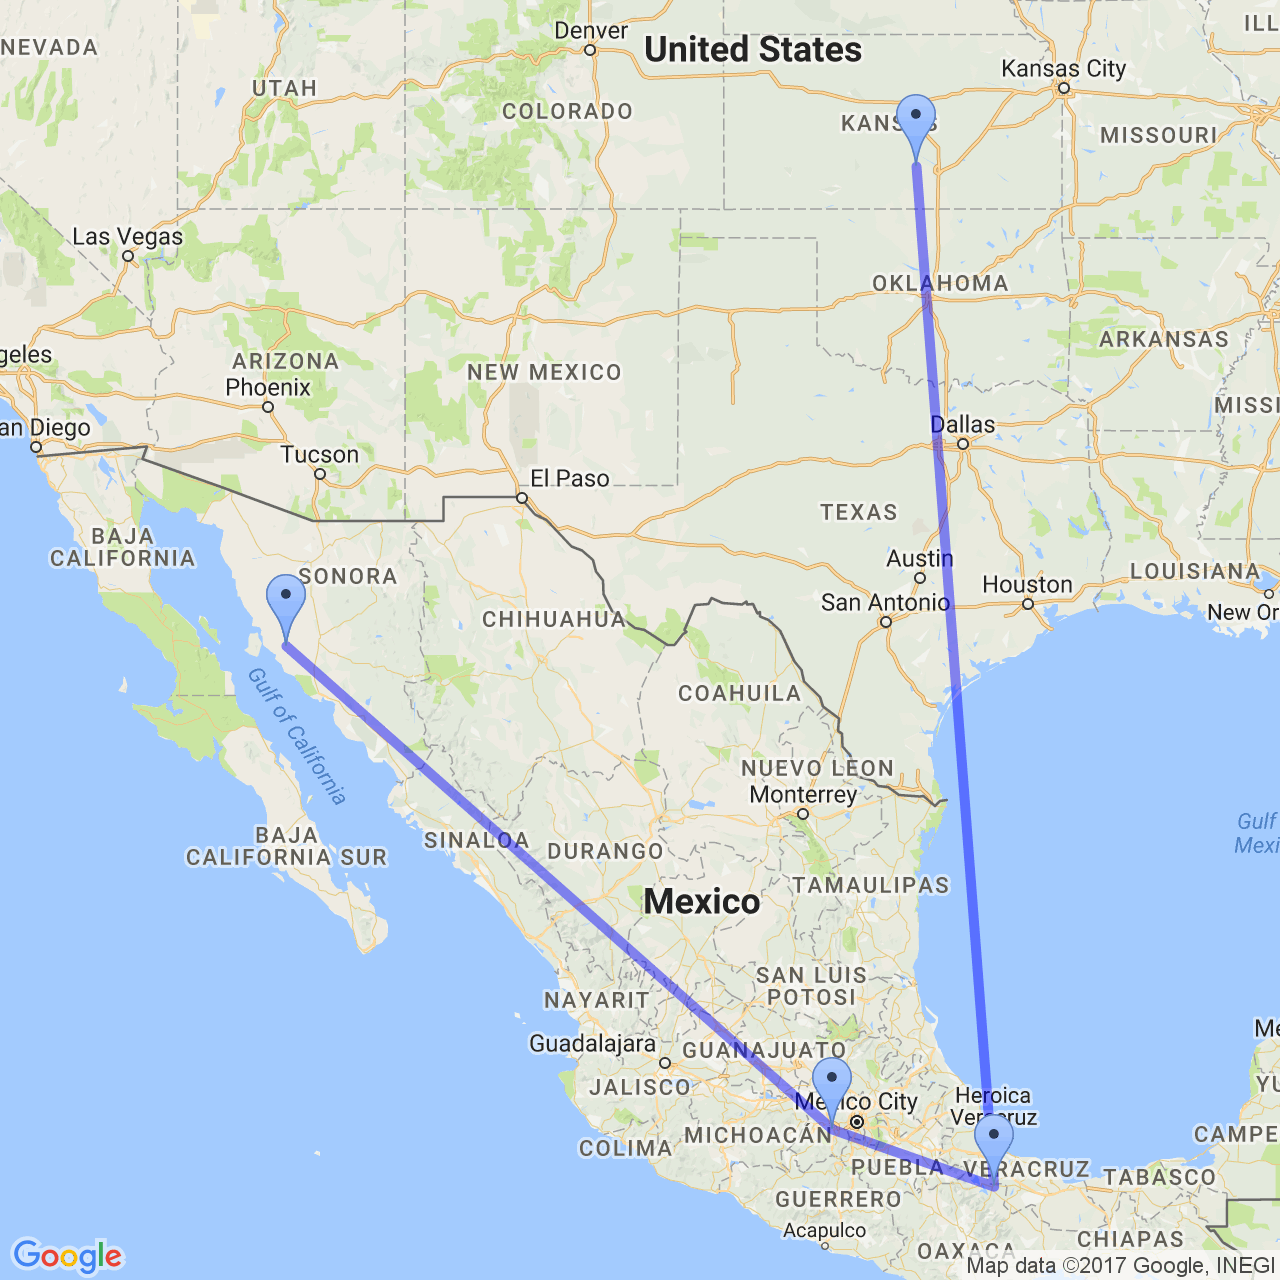
\includegraphics[width=0.55\textwidth]{modules/unam_path_2}
 \label{fig:ruta_unam_2}
\end{figure}

\newpage

\subsection{Europa}


\newpage
\subsection{UK}


\newpage



\newpage

\section{Conclusión}



\newpage
\section{Conclusión}

 
\begin{thebibliography}{9}
\bibitem{Scapy} 
\texttt{www.secdev.org/projects/scapy/}

\bibitem{ICMP} 
\texttt{http://www.ietf.org/rfc/rfc792.txt}

\bibitem{Cimbala} 
\texttt{http://www.mne.psu.edu/cimbala/me345/Lectures/Outliers.pdf
}
\bibitem{GeoIP}
\texttt{http://www.geoiptool.com/es/}

\bibitem{Anomalias}
\texttt{$http://www.net.in.tum.de/fileadmin/TUM/NET/NET-2012-08-1/
NET-2012-08-1_02.pdf$}

\end{thebibliography}

\newpage


%\input{others/comentarios}

\end{document}
